\documentclass[11pt]{article}
\usepackage{geometry, titlesec}
\usepackage[parfill]{parskip}
\usepackage[italicdiff]{physics}
\usepackage{amsfonts, amsthm}
\usepackage[cm]{fullpage}
\usepackage{fancyhdr}
\usepackage{enumitem}
\usepackage{xcolor, soul}
\usepackage{graphicx}
\usepackage[export]{adjustbox}
\usepackage{siunitx}
%\allowdisplaybreaks

\renewcommand{\thesubsection}{\thesection.\alph{subsection}}
\setenumerate[1]{label={(\alph*)}}

\makeatletter
\renewcommand*\env@cases[1][1.2]{%
  \let\@ifnextchar\new@ifnextchar
  \left\lbrace
  \def\arraystretch{#1}%
  \array{@{}l@{\quad}l@{}}%
}
\makeatother
 
\renewcommand{\footrulewidth}{.2pt}
%\setlist[enumerate]{leftmargin=*}
\pagestyle{fancy}
\fancyhf{}
\lhead{Physics 132-B}
\chead{\textbf{Discussion 4 Problems}}
\rhead{A--De Discussion}
\setlength{\headheight}{11pt}
\setlength{\headsep}{11pt}
\setlength{\footskip}{24pt}
\lfoot{\today}
\rfoot{\thepage}

\titleformat{\subsection}[runin]{\normalfont\large\bfseries}{\thesubsection}{1em}{}
\newcommand{\refeq}[1]{(\ref{#1})}

\newcommand{\beq}{\begin{equation*}}
\newcommand{\eeq}{\end{equation*}}

\newcommand{\beqn}{\begin{equation}}
\newcommand{\eeqn}{\end{equation}}

\newcommand{\blg}{\begin{align*}}
\newcommand{\elg}{\end{align*}}


\newenvironment{statement}
{
%    \color{gray}
    \ignorespaces
}
{
%    \smallskip
}

\newenvironment{problem}
{
    \color{darkgray}
    \ignorespaces
}

\newenvironment{solution}
{
    \paragraph{Solution.}
    \ignorespaces
}
{
    \bigskip
}

\renewcommand{\vec}[1]{\mathbf{#1}}


\begin{document}
	

\newcommand{\vE}{\vec{E}}

\begin{minipage}[l]{0.65\textwidth}
%\paragraph{Problem 21.96}
\paragraph{Problem 1}
\begin{problem}
	Two charges are placed as shown in Fig.~1.  The magnitude of $q_1$ is \SI{3.00}{\micro\coulomb}, but its sign and the value of the charge $q_2$ are not known.  The direction of the net electric field $\vE$ at point $P$ is entirely in the negative $y$ direction. \medskip
	\begin{enumerate}
		\item Considering the different possible signs of $q_1$ and $q_2$, four possible diagrams could represent the electric fields $\vE_1$ and $\vE_2$ produced by $q_1$ and $q_2$.  Sketch the four possible electric field configurations.\medskip
		\item Using the sketches from part (a) and the direction of $\vE$, deduce the signs of $q_1$ and $q_2$.\medskip
		\item Determine the magnitude of $\vE$.
	\end{enumerate}
\end{problem}
\end{minipage}%
\hspace{0.05\textwidth}%
\begin{minipage}[r]{0.3\textwidth}
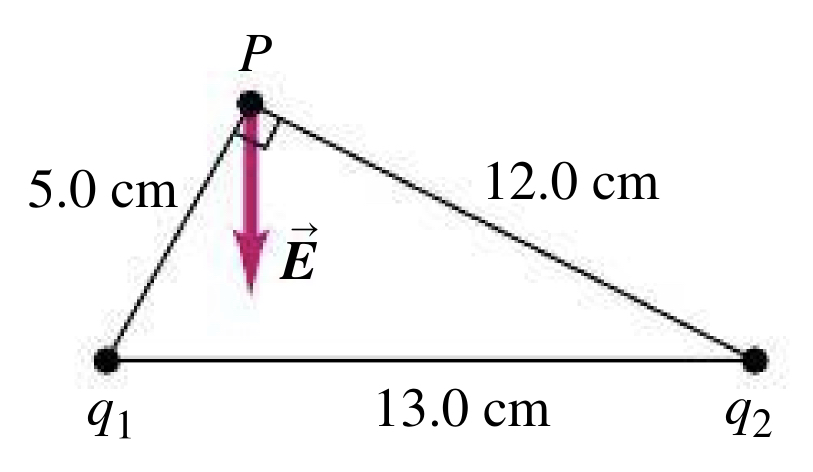
\includegraphics[width=\textwidth]{P21-96.jpeg}
\center \textbf{Figure 1}
\end{minipage}

\vfill
	
%\paragraph{Problem 23.82}
\paragraph{Problem 2}
\begin{problem}
	A hollow, thin-walled insulating cylinder of radius $R$ and length $L$ (like the cardboard tube in a roll of toilet paper) has charge $Q$ uniformly distributed over its surface.
	
	\begin{enumerate}
		\item Calculate the electric potential at all points along the axis of the tube.  Take the origin to be at the center of the tube, and take the potential to be zero at infinity.
		\item Use the result of part (a) to find the electric field at all points along the axis of the tube.
	\end{enumerate}
\end{problem}

\vfill


\clearpage

\begin{minipage}[b]{0.65\textwidth}
%\paragraph{Problem 22.34}
\paragraph{Problem 3}
\begin{problem}
	A cube has sides of length $L = \SI{0.350}{\meter}$.  One corner is at the origin~(Fig.~2).  The nonuniform electric field is given by ${\vE = (\SI{-5.64}{\newton\per\coulomb\per\meter})x \, \vec{\hat{i}} + (\SI{2.54}{\newton\per\coulomb\per\meter}) z \, \vec{\hat{k}}}$. \medskip
	\begin{enumerate}
		\item Find the electric flux through each of the six cube faces $S_1,\ S_2,\ S_3,\ S_4,\ S_5$, and $S_6$. \medskip
		\item Find the total electric charge inside the cube.
	\end{enumerate}
\end{problem}
\end{minipage}%
\hspace{0.05\textwidth}%
\begin{minipage}{0.3\textwidth}
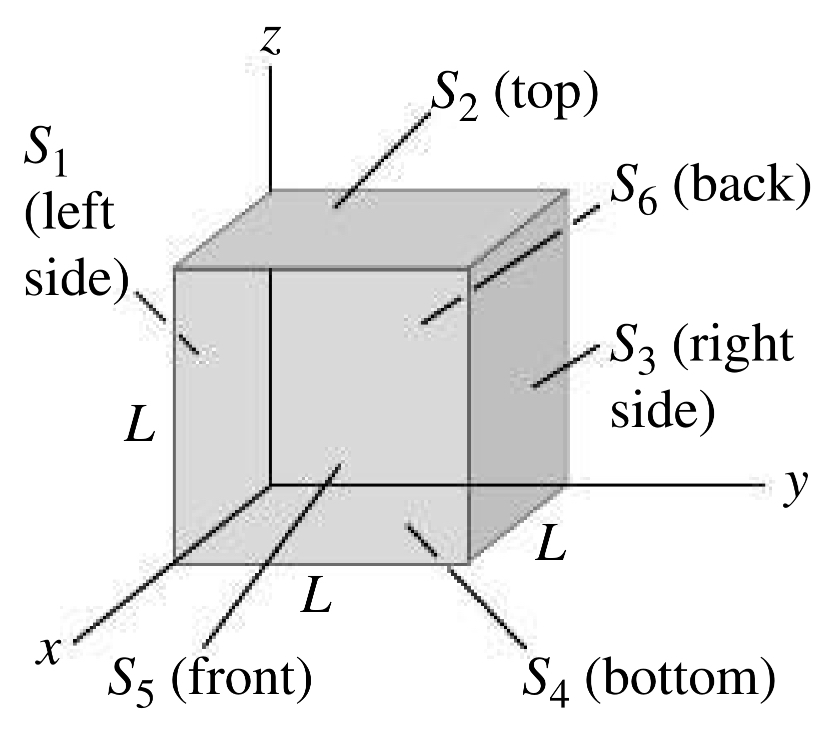
\includegraphics[width=\textwidth]{E22-6.jpeg}
\center \textbf{Figure 3}
\end{minipage}

\vspace{-6\baselineskip}
\vfill

\paragraph{Problem 4}
%\paragraph{Problem 24.11}
\begin{problem}
	A spherical capacitor contains a charge of \SI{3.10}{\nano\coulomb} when connected to a potential difference of \SI{240}{\volt}.  If its plates are separated by vacuum and the inner radius of the outer shell is \SI{4.40}{\centi\meter}, calculate
	
	\begin{enumerate}
		\item the capacitance,
		\item the radius of the inner sphere, and
		\item the electric field just outside the surface of the inner sphere.
	\end{enumerate}
\end{problem}

\vfill

\end{document}